\chapter{Lab 4: Hex Calculator \\
\index{Lab 4}
\index{introduction}
\label{Introduction}}


\section{Lessons Learned
    We learned how to use the buttons on the board to perform different functions. This would be useful for our final project so we will take the pad to try and utilize the number pad to control the blocks. 
\label{Section::Lessons Learned}}
 \section{Schematics and Block Diagrams}
    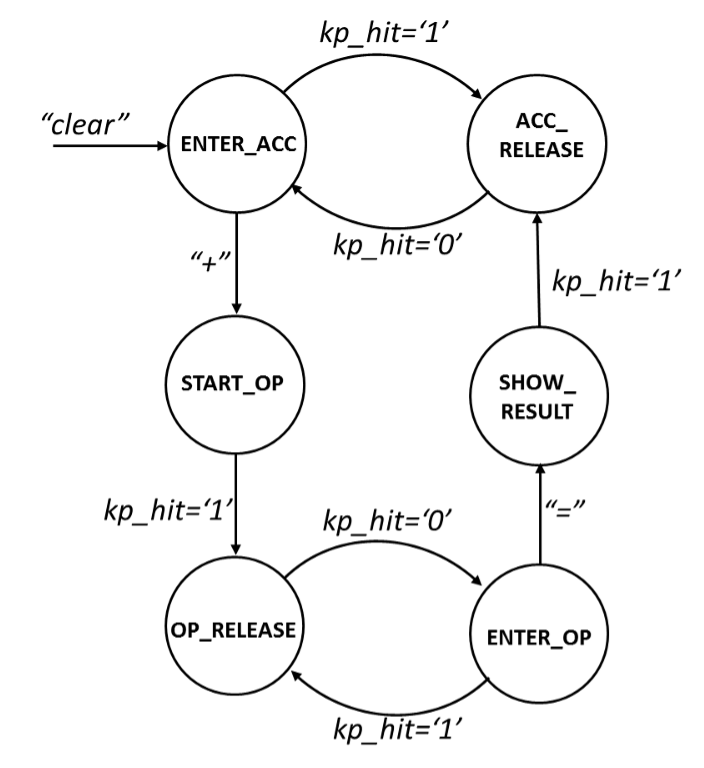
\includegraphics[width=100mm]{lab4/hexcalc.png}
    \emph{Figure 4.1: Input and Output of the System}
    
 \section{VHDL Architecture}
 \begin{verbatim}
     ## Clock signal
    set_property -dict { PACKAGE_PIN E3    IOSTANDARD LVCMOS33 } [get_ports { clk_50MHz }]; #IO_L12P_T1_MRCC_35 Sch=clk100mhz
    create_clock -add -name sys_clk_pin -period 10.00 -waveform {0 5} [get_ports {clk_50MHz}];

    ##Buttons

    #set_property -dict { PACKAGE_PIN C12   IOSTANDARD LVCMOS33 } [get_ports { CPU_RESETN }]; #IO_L3P_T0_DQS_AD1P_15 Sch=cpu_resetn

    set_property -dict { PACKAGE_PIN N17   IOSTANDARD LVCMOS33 } [get_ports { bt_clr }]; #IO_L9P_T1_DQS_14 Sch=btnc
    set_property -dict { PACKAGE_PIN M18   IOSTANDARD LVCMOS33 } [get_ports { bt_plus }]; #IO_L4N_T0_D05_14 Sch=btnu
    set_property -dict { PACKAGE_PIN P17   IOSTANDARD LVCMOS33 } [get_ports { bt_eq }]; #IO_L12P_T1_MRCC_14 Sch=btnl
    #set_property -dict { PACKAGE_PIN M17   IOSTANDARD LVCMOS33 } [get_ports { BTNR }]; #IO_L10N_T1_D15_14 Sch=btnr
    set_property -dict { PACKAGE_PIN P18   IOSTANDARD LVCMOS33 } [get_ports { bt_sub }]; #IO_L9N_T1_DQS_D13_14 Sch=btnd

    ##Pmod Header JA

    set_property -dict { PACKAGE_PIN C17   IOSTANDARD LVCMOS33 } [get_ports { KB_col[4] }]; #IO_L20N_T3_A19_15 Sch=ja[1]
    set_property -dict { PACKAGE_PIN D18   IOSTANDARD LVCMOS33 } [get_ports { KB_col[3] }]; #IO_L21N_T3_DQS_A18_15 Sch=ja[2]
    set_property -dict { PACKAGE_PIN E18   IOSTANDARD LVCMOS33 } [get_ports { KB_col[2] }]; #IO_L21P_T3_DQS_15 Sch=ja[3]
    set_property -dict { PACKAGE_PIN G17   IOSTANDARD LVCMOS33 } [get_ports { KB_col[1] }]; #IO_L18N_T2_A23_15 Sch=ja[4]
    set_property -dict { PACKAGE_PIN D17   IOSTANDARD LVCMOS33 } [get_ports { KB_row[4] }]; #IO_L16N_T2_A27_15 Sch=ja[7]
    set_property -dict { PACKAGE_PIN E17   IOSTANDARD LVCMOS33 } [get_ports { KB_row[3] }]; #IO_L16P_T2_A28_15 Sch=ja[8]
    set_property -dict { PACKAGE_PIN F18   IOSTANDARD LVCMOS33 } [get_ports { KB_row[2] }]; #IO_L22N_T3_A16_15 Sch=ja[9]
    set_property -dict { PACKAGE_PIN G18   IOSTANDARD LVCMOS33 } [get_ports { KB_row[1] }]; #IO_L22P_T3_A17_15 Sch=ja[10]

    ##7-Segment Display
    set_property -dict {PACKAGE_PIN L18 IOSTANDARD LVCMOS33} [get_ports {SEG7_seg[0]}]
    set_property -dict {PACKAGE_PIN T11 IOSTANDARD LVCMOS33} [get_ports {SEG7_seg[1]}]
    set_property -dict {PACKAGE_PIN P15 IOSTANDARD LVCMOS33} [get_ports {SEG7_seg[2]}]
    set_property -dict {PACKAGE_PIN K13 IOSTANDARD LVCMOS33} [get_ports {SEG7_seg[3]}]
    set_property -dict {PACKAGE_PIN K16 IOSTANDARD LVCMOS33} [get_ports {SEG7_seg[4]}]
    set_property -dict {PACKAGE_PIN R10 IOSTANDARD LVCMOS33} [get_ports {SEG7_seg[5]}]
    set_property -dict {PACKAGE_PIN T10 IOSTANDARD LVCMOS33} [get_ports {SEG7_seg[6]}]

    set_property -dict {PACKAGE_PIN U13 IOSTANDARD LVCMOS33} [get_ports {SEG7_anode[7]}]
    set_property -dict {PACKAGE_PIN K2 IOSTANDARD LVCMOS33} [get_ports {SEG7_anode[6]}]
    set_property -dict {PACKAGE_PIN T14 IOSTANDARD LVCMOS33} [get_ports {SEG7_anode[5]}]
    set_property -dict {PACKAGE_PIN P14 IOSTANDARD LVCMOS33} [get_ports {SEG7_anode[4]}]
    set_property -dict {PACKAGE_PIN J14 IOSTANDARD LVCMOS33} [get_ports {SEG7_anode[3]}]
    set_property -dict {PACKAGE_PIN T9 IOSTANDARD LVCMOS33} [get_ports {SEG7_anode[2]}]
    set_property -dict {PACKAGE_PIN J18 IOSTANDARD LVCMOS33} [get_ports {SEG7_anode[1]}]
    set_property -dict {PACKAGE_PIN J17 IOSTANDARD LVCMOS33} [get_ports {SEG7_anode[0]}]
 \end{verbatim}
 \section{VHDL Models}
 \begin{itemize}
     \item Data Flow
        \begin{verbatim}
            hexcalc.vhd
                input: clock at 50 MHz, calculator functions ('+', '=', '-', and 'clear')
                output: keyboard column pins 
            keyboard.vhd
                input: row lines
                output: hex value of a key press, column lines
            leddec16.vhd
                input: digit display, and 16 digit data
                output: anode display, segment code for each digit
        \end{verbatim}
     \item Structural
        \begin{verbatim}
            hexcalc
                kp1 : keypad
                led1 : leddec16
        \end{verbatim}
     \item Behavioral
        The program inputs are primarily coming from the 16-button keypad module and buttons on the FPGA board. The keypad dictates what values are used which is displayed on the board's LEDs and then the buttons on the board dictate whether it is adding or subtraction. After the calculator portion the answer is displayed on the board. 
\end{itemize}
 \section{VHDL Component Reuse}
    This section reuses the LED section from Labs 1 and 2 and then combined them together with using the button to make a hexadecimal calculator.
 \section{VHDL Digital Circuits}
    
 \section{State Machines}
    The system is idle until a button is pressed on the key pad and then displays the number on the LED bank and then returns to idle until another number is pushed or a function button is pressed. Then after pushing the enter button, the board displays the answer and then returns to idle state. 
 \section{Testing}
    We tested this by inputting different numbers on the pad. We did notice that if you cause a negative number on the pad, it overflows and fills the entire LED bank. We added and subtracted random numbers to see how the board would respond to different inputs. 
